	\begin{figure}[H]
		\centering
 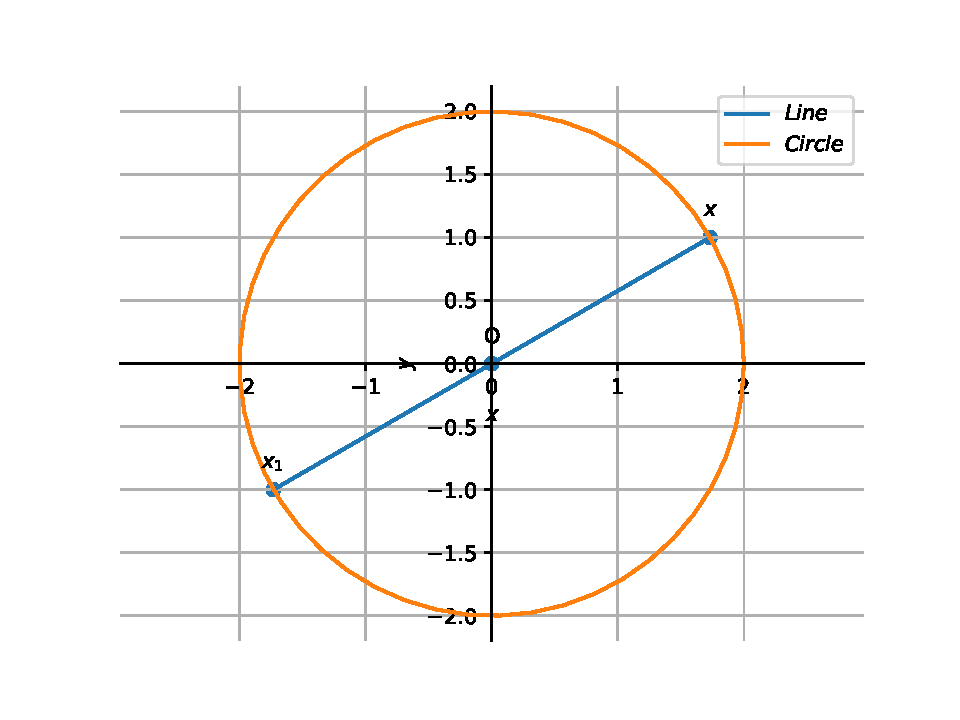
\includegraphics[width=0.75\columnwidth]{chapters/12/8/1/6/figs/conics-fig.pdf} 
		\caption{}
		\label{fig:12/8/1/6}
  	\end{figure}
  From the given information, the parameters of the  circle and line are
                      \begin{align}
			      f= -4, \vec{u}=\vec{0}, \vec{V}=\vec{I}, \vec{m}=\myvec{1 \\ \sqrt{3}}, \vec{h} = \vec{0}
		\label{eq:12/8/1/6}
                    \end{align}                                                                              
Substituting		    the above parameters in  
\eqref{eq:tangent_roots},
	  \begin{align}                                                                               
		  \mu= \sqrt{3}
	  \end{align}
	  yielding  
the desired point of intersection as                                               
\begin{align}
	\vec{x} = \myvec{\sqrt{3} \\ 1}                               
\end{align}
Note that we have chosen only the point of intersection in the first quadrant as shown in 
		\figref{fig:12/8/1/6}.
From
		\eqref{eq:12/8/1/6},
		the angle between the given line and the x axis is
\begin{align}
	\theta=30\degree
\end{align} 
and
the area of the sector is 
\begin{align}
	{\frac{\theta}{360}}\pi r^2=
	\frac{\pi}{3}
\end{align}
